\documentclass[aspectratio=169,11pt]{beamer}

% ================================================================
% "TABIIY TILNI QAYTA ISHLASH" KURSI
% MA'RUZA 13 --- Transfer Learning va oldindan o'qitilgan modellar (BERT, T5)
%              (d13_transfer_learning.tex)
% Arxetiplar: [A][B][C][D][E] + 4 tsikl [F][G][H][I][J][K][L] +
%             [M][N][O][P][Q][R] + ilova [S]
% Rendered slayd soni: ~45 (4-haftaning birinchi ma'ruzasi; L1-L12 chuqurligi)
% Qulflangan [I1]: sigma(2.0)=0.880, BCE=0.128
%   --- P13 (Day 14) birinchi assert manbayi (course_map hand_example).
% MUHIM ARK: L12 Transformer -> L13 BERT (enkoder) / T5 (enkoder-dekoder) ustiga qurilgan.
% ================================================================

% ================================================================
% RANGLAR  (asl fayldan o'zgarishsiz)
% ================================================================
\definecolor{cnublue}{rgb}{0.07,0.14,0.62}
\definecolor{cnubluelight}{rgb}{0.18,0.30,0.72}
\definecolor{cnubluebg}{rgb}{0.90,0.92,0.97}
\definecolor{deepblue}{rgb}{0.07,0.14,0.62}
\definecolor{deepred}{rgb}{0.60,0.00,0.00}
\definecolor{deepgreen}{rgb}{0.00,0.45,0.00}
\definecolor{halfgray}{gray}{0.55}

% ================================================================
% BEAMER MAVZU --- Boadilla + maxsus footer  (asl fayldan o'zgarishsiz)
% ================================================================
\usetheme{Boadilla}

\setbeamercolor{structure}{fg=cnublue}
\setbeamercolor{frametitle}{bg=cnublue,fg=white}
\setbeamercolor{title}{bg=cnublue,fg=white}
\setbeamercolor{block title}{bg=cnublue,fg=white}
\setbeamercolor{block body}{bg=cnubluebg,fg=black}
\setbeamercolor{alerted text}{fg=deepred}
\setbeamercolor{author in head/foot}{bg=cnubluelight,fg=white}
\setbeamercolor{section in head/foot}{bg=cnublue,fg=white}
\setbeamercolor{page number in head/foot}{bg=cnubluelight,fg=white}

\setbeamertemplate{mini frame}{}
\setbeamertemplate{mini frame in current section}{}
\setbeamertemplate{mini frame in current subsection}{}
\setbeamertemplate{headline}{}
\setbeamertemplate{navigation symbols}{}

\setbeamertemplate{footline}{%
  \leavevmode%
  \hbox{%
    \begin{beamercolorbox}[wd=0.17\paperwidth,ht=2.5ex,dp=1.25ex,leftskip=0.5em]{author in head/foot}%
      \usebeamerfont{author in head/foot}\scriptsize\insertshortauthor%
    \end{beamercolorbox}%
    \begin{beamercolorbox}[wd=0.69\paperwidth,ht=2.5ex,dp=1.25ex,center]{section in head/foot}%
      \usebeamerfont{section in head/foot}%
      \scriptsize\insertsectionnavigationhorizontal{0.69\paperwidth}{}{}%
    \end{beamercolorbox}%
    \begin{beamercolorbox}[wd=0.14\paperwidth,ht=2.5ex,dp=1.25ex,rightskip=0.5em]{page number in head/foot}%
      \hfill\scriptsize\color{white}%
      \insertframenumber{}/\inserttotalframenumber%
    \end{beamercolorbox}%
  }%
  \vskip0pt%
}

% ================================================================
% PAKETLAR  (asl fayldan o'zgarishsiz)
% ================================================================
\usepackage[utf8]{inputenc}
\usepackage[T1]{fontenc}
\usepackage{lmodern}
\usepackage{amsmath,amssymb}
\usepackage{booktabs}
\usepackage{xcolor}
\usepackage{listings}
\lstset{
    language=Python,
    basicstyle=\ttfamily\scriptsize,
    keywordstyle=\bfseries\color{deepblue},
    emphstyle=\ttfamily\color{deepred},
    stringstyle=\color{deepgreen},
    commentstyle=\itshape\color{halfgray},
    numbers=left,
    numberstyle=\scriptsize\color{halfgray},
    rulesepcolor=\color{cnublue!30},
    frame=shadowbox,
    breaklines=true,
    showstringspaces=false,
    tabsize=2
}
\usepackage{tcolorbox}
\tcbuselibrary{skins}
\tcbset{
  defbox/.style={colback=cnubluebg,colframe=cnublue,
                 fonttitle=\small\bfseries\color{white},
                 attach boxed title to top left={yshift=-2mm,xshift=4mm},
                 boxed title style={colback=cnublue,colframe=cnublue}},
  warnbox/.style={colback=orange!8,colframe=orange!70!black,
                  fonttitle=\small\bfseries},
  okbox/.style={colback=green!7,colframe=green!55!black,
                fonttitle=\small\bfseries}
}
\usepackage{tikz}
\usetikzlibrary{arrows.meta,positioning}

% ================================================================
% QO'SHIMCHALAR  (asl fayldan o'zgarishsiz)
% ================================================================
\AtBeginSection[]{%
  \begin{frame}{Prezentatsiya rejasi}
    \tableofcontents[currentsection]
  \end{frame}}

\newcommand{\bunda}[1]{{\small\textbf{bunda:}\; #1}}
\newcommand{\bajarildi}{{\color{deepgreen}\large$\checkmark$}\;}

% ================================================================
% METAMA'LUMOT
% ================================================================
\title[Transfer Learning]{Transfer Learning va oldindan o'qitilgan modellar\\ (BERT, T5)}
\subtitle{Tabiiy tilni qayta ishlash --- 13-ma'ruza}
\author[A.A.\,Abdulali]{A.A.\,Abdulali}
\date{6-iyul 2026}
\institute{11:00--12:20 \quad$\cdot$\quad mavzu \textnumero{}13}

% ================================================================
\begin{document}
% ================================================================

% ----------------------------------------------------------------
% [A] TITUL
% ----------------------------------------------------------------
\maketitle

% ================================================================
\section[Kirish]{Kirish: noldan o'qitmaymiz, oldindan o'qitilganni olamiz}
% ================================================================

% ----------------------------------------------------------------
% [B] TAKRORLASH: L12 va bugungi P12
% ----------------------------------------------------------------
\begin{frame}{Takrorlash: o'tgan darsdan ikki savol}
  \begin{columns}[T]
    \begin{column}{0.49\textwidth}
      \begin{tcolorbox}[warnbox,title=1-savol]
        \small
        L12 da Transformer'ni quridik. Uni o'qitish uchun nima kerak edi ---
        qancha ma'lumot va hisob?
      \end{tcolorbox}
    \end{column}
    \begin{column}{0.49\textwidth}
      \begin{tcolorbox}[warnbox,title=2-savol]
        \small
        O'zbek tili uchun millionlab yorliqlangan namuna yo'q. Unda kuchli
        Transformer'ni qanday quramiz?
      \end{tcolorbox}
    \end{column}
  \end{columns}
  \pause
  \vspace{4pt}
  \begin{columns}[T]
    \begin{column}{0.49\textwidth}
      \begin{tcolorbox}[okbox,title=1-javob]
        \small
        Juda ko'p: katta korpus, ko'p GPU, kunlab o'qitish. Noldan har safar
        bu --- isrof.
      \end{tcolorbox}
    \end{column}
    \begin{column}{0.49\textwidth}
      \begin{tcolorbox}[okbox,title=2-javob]
        \small
        \textbf{Oldindan o'qitilgan} modelni olamiz va kichik datada
        \textbf{sozlaymiz} (fine-tuning) --- bugungi mavzu: transfer learning.
      \end{tcolorbox}
    \end{column}
  \end{columns}
\end{frame}

% ----------------------------------------------------------------
% [C] MAQSADLAR
% ----------------------------------------------------------------
\begin{frame}{Siz bugungi dars oxirida quyidagilarni bajara olasiz:}
  \begin{enumerate}\setlength\itemsep{6pt}
    \item \textbf{Tushuntira olasiz:} transfer learning --- pre-training va
          fine-tuning farqi va nega kam-resursli til uchun zarur.
    \item \textbf{Hisoblay olasiz:} fine-tuning BCE yo'qotishini ---
          $\sigma(2.0)\approx 0.880$, $\mathrm{BCE}\approx 0.128$.
    \item \textbf{Tushuntira olasiz:} BERT (ikki tomonlama enkoder, MLM) va
          T5 (matn$\to$matn) farqini.
    \item \textbf{Tushuntira olasiz:} Hugging Face ekotizimi bilan fine-tuning oqimini.
  \end{enumerate}
  \vspace{4pt}
  \begin{tcolorbox}[defbox,title=Oldindan talab]
    \footnotesize
    L12 dan: Transformer, self-attention. L2 dan: logistik regressiya, sigmoid.
    L6/L9 dan: softmax. Matematikadan: $\exp$, $\ln$, ehtimol.
  \end{tcolorbox}
\end{frame}

% ----------------------------------------------------------------
% [D] REJA
% ----------------------------------------------------------------
\begin{frame}{Bugungi dars rejasi:}
  \begin{center}
  \small
  \begin{tabular}{c p{5.2cm} c p{3.0cm}}
    \toprule
    \textbf{Tsikl}& \textbf{Mavzu} & \textbf{Vaqt} & \textbf{Hosil bo'luvchi natija}\\
    \midrule
    1 & Transfer learning va fine-tuning & 16 daq & BCE $=0.128$ \\
    2 & BERT: ikki tomonlama enkoder & 16 daq & MLM bashorati \\
    3 & T5: matndan matnga & 16 daq & yagona format \\
    4 & Hugging Face ekotizimi & 16 daq & fine-tuning oqimi \\
    \midrule
      & Xulosa va 13-amaliyotga ko'rsatmalar & 10 daq & Ertaga nima qurishingiz \\
    \bottomrule
  \end{tabular}
  \end{center}
  \vspace{4pt}
  \begin{tcolorbox}[warnbox,title=Bu dars fine-tuning'ga olib keladi]
    \footnotesize\sloppy
    Oldindan o'qitilgan modelni kichik datada sozlaymiz. Bugungi
    $\mathrm{BCE}=0.128$ ertangi P13 da \texttt{assert} bo'ladi.
  \end{tcolorbox}
\end{frame}

% ----------------------------------------------------------------
% [E] MUAMMO BIRINCHI
% ----------------------------------------------------------------
\begin{frame}{Bugungi dars uchun muammo: noldan o'qitish kam-resursli til uchun imkonsiz}
  \begin{columns}[T]
    \begin{column}{0.50\textwidth}
      \textbf{Noldan o'qitish qayerda qiynaladi:}\\[3pt]
      \small
      \begin{tcolorbox}[warnbox,title={Ulkan ma'lumot talabi},top=2pt,bottom=2pt]
        \footnotesize
        Kuchli Transformer milliardlab so'z va minglab GPU-soat talab qiladi.
        O'zbek uchun bunday yorliqlangan korpus yo'q.
      \end{tcolorbox}
      \vspace{3pt}
      \begin{tcolorbox}[warnbox,title={Har vazifaga qaytadan},top=2pt,bottom=2pt]
        \footnotesize
        Sentiment, NER, tarjima --- har biri uchun noldan o'qitish ulkan isrof.
      \end{tcolorbox}
    \end{column}
    \begin{column}{0.46\textwidth}
      \textbf{Bugungi yechim:}\\[4pt]
      \small
      \begin{enumerate}\setlength\itemsep{4pt}
        \item Katta korpusda \textbf{bir marta} oldindan o'qitilgan model
              (umumiy til bilimi).
        \item Uni \textbf{kichik} yorliqlangan datada \textbf{sozlaymiz}
              (fine-tuning).
        \item Bilim \textbf{ko'chiriladi} (transfer) --- kam data, kam hisob.
      \end{enumerate}
      \vspace{5pt}
      \begin{tcolorbox}[okbox,top=2pt,bottom=2pt]
        \footnotesize
        BERT, T5 --- L12 dagi Transformer ustiga qurilgan, oldindan o'qitilgan
        modellar. Biz ularni olamiz.
      \end{tcolorbox}
    \end{column}
  \end{columns}
\end{frame}

% ================================================================
\section[Transfer]{Transfer learning: pre-training va fine-tuning}
% ================================================================

% ----------------------------------------------------------------
% [F1] INTUITSIYA
% ----------------------------------------------------------------
\begin{frame}{Intuitsiya: avval umumiy o'rgan, keyin vazifaga moslan}
  \begin{columns}[T]
    \begin{column}{0.52\textwidth}
      \small
      Inson ham tilni avval umumiy o'rganadi, keyin aniq kasbga moslashtiradi.
      Model ham:
      \begin{itemize}\setlength\itemsep{1pt}
        \item \textbf{Pre-training}: katta yorliqsiz korpusda umumiy til bilimi
              (o'z-o'zini nazorat).
        \item \textbf{Fine-tuning}: kichik yorliqlangan datada aniq vazifaga
              sozlash (nazorat ostida).
      \end{itemize}
    \end{column}
    \begin{column}{0.44\textwidth}
      \begin{tcolorbox}[okbox,top=2pt,bottom=2pt]
        \footnotesize
        Oldindan o'qitilgan vaznlar --- yaxshi \textbf{boshlang'ich nuqta}.
        Fine-tuning ularni biroz suradi, noldan boshlamaydi.
      \end{tcolorbox}
    \end{column}
  \end{columns}
\end{frame}

% ----------------------------------------------------------------
% [G1] RASMIY TA'RIF + BUNDA
% ----------------------------------------------------------------
\begin{frame}{Fine-tuning yo'qotishi: rasmiy ta'rif}
  \begin{tcolorbox}[defbox,title={Ta'rif: sigmoid va BCE (ikkilik klassifikatsiya)}]
    \vspace{-0.4em}
    $$ p = \sigma(z) = \frac{1}{1+e^{-z}}, \qquad
       \mathrm{BCE} = -\big[\,y\ln p + (1-y)\ln(1-p)\,\big] $$
  \end{tcolorbox}
  \vspace{2pt}
  \bunda{$z$ --- model logiti (oxirgi qatlam chiqishi); $p$ --- ijobiy sinf
  ehtimoli; $y\in\{0,1\}$ --- haqiqiy yorliq (ijobiy $=1$, salbiy $=0$);
  $\mathrm{BCE}$ --- ikkilik kross-entropiya yo'qotishi.}
  \vspace{4pt}
  \footnotesize Fine-tuning bu yo'qotishni kichik yorliqlangan datada
  minimallashtiradi --- oldindan o'qitilgan vaznlardan boshlab.
\end{frame}

% ----------------------------------------------------------------
% [H1] KELTIRIB CHIQARISH
% ----------------------------------------------------------------
\begin{frame}{Keltirib chiqarish: nega avval pre-train, keyin fine-tune?}
  \textbf{1-qadam.} Tasodifiy boshlang'ich vaznlar juda ko'p yorliqlangan
  ma'lumot talab qiladi --- o'zbek uchun yo'q.
  \pause
  \textbf{2-qadam.} Yorliqsiz katta korpusda o'z-o'zini nazorat (masalan, niqoblangan
  so'zni bashorat) --- bu ma'lumot \textbf{ko'p va arzon}.
  \pause
  \textbf{3-qadam.} Model umumiy til naqshlarini o'rganadi --- yaxshi boshlang'ich
  vaznlar.
  \pause
  \textbf{4-qadam.} Kichik yorliqlangan datada faqat \textbf{sozlaymiz} --- BCE
  ni minimallashtiramiz, kam qadamda.
  \begin{tcolorbox}[okbox,top=2pt,bottom=2pt]
    \small \textbf{Xulosa:} pre-training bilimni beradi, fine-tuning uni
    vazifaga buradi. Endi BCE'ni qo'lda hisoblaymiz.
  \end{tcolorbox}
\end{frame}

% ----------------------------------------------------------------
% [I1] QO'LDA HISOB --- QULFLANGAN TRACEABILITY SLAYD
%
% P13 (Day 14) birinchi assert bilan solishtiring:
%   sigma(2.0)=0.880, BCE=0.128   [Ma'ruza L13 [I1]-slayd]
% course_map.yaml hand_example verbatim.
% ----------------------------------------------------------------
\begin{frame}{Qo'lda hisob: sigmoid va BCE yo'qotishi $=0.128$}
  \begin{tcolorbox}[defbox,title={Ijobiy sharh, logit $z=2.0$, yorliq $y=1$}]
    \small $e^{-2.0}\approx 0.135$.
  \end{tcolorbox}
  \vspace{0.2em}
  \begin{columns}[T]
    \begin{column}{0.54\textwidth}
      \textbf{Sigmoid va BCE:}
      \begin{align*}
        p &= \sigma(2.0) = \tfrac{1}{1+0.135} = \tfrac{1}{1.135} \approx \mathbf{0.880}\\
        \mathrm{BCE} &= -\ln(0.880) \approx \mathbf{0.128}
      \end{align*}
    \end{column}
    \begin{column}{0.42\textwidth}
      \begin{tcolorbox}[okbox,top=2pt,bottom=2pt]
        \footnotesize
        Model ijobiy sinfga $0.880$ ishonch berdi; yorliq ham ijobiy
        $\Rightarrow$ \textbf{past} yo'qotish ($0.128$).
      \end{tcolorbox}
      \vspace{3pt}
      \footnotesize\color{halfgray}
      Ertangi P13 birinchi assert:\\
      \texttt{assert abs(loss - 0.128)}\\
      \texttt{\phantom{xx}< 1e-2}\\
      \textit{\# Ma'ruza L13 [I1]-slayd}
    \end{column}
  \end{columns}
\end{frame}

% ----------------------------------------------------------------
% [J1] SIZNING VAZIFANGIZ
% ----------------------------------------------------------------
\begin{frame}{Sizning vazifangiz: nol logit uchun BCE}
  \begin{tcolorbox}[warnbox,title=Savol --- 60 soniya]
    \small
    Model ishonchsiz: logit $z=0.0$, yorliq $y=1$ (ijobiy). $\sigma(0)=0.5$.\\[4pt]
    \textbf{\large $\mathrm{BCE} = -\ln(0.5) = ?$} \quad
    \footnotesize ($\ln 2 \approx 0.693$)
  \end{tcolorbox}
  \pause
  \begin{tcolorbox}[okbox,title=Javob]
    \small
    $\mathrm{BCE} = -\ln(0.5) = \ln 2 \approx \mathbf{0.693}$\\[3pt]
    \footnotesize Ishonchsiz bashorat (50/50) yo'qotishi $0.693$ --- ishonchli
    to'g'ri ($0.128$) dan ancha yuqori. Fine-tuning buni pasaytiradi.
  \end{tcolorbox}
\end{frame}

% ----------------------------------------------------------------
% [K1] KOD <-> FORMULA  [fragile]
% ----------------------------------------------------------------
\begin{frame}[fragile]{Kod $\leftrightarrow$ formula: BCE yo'qotishi}
  \begin{columns}[T]
    \begin{column}{0.58\textwidth}
\begin{lstlisting}
import torch
import torch.nn as nn

logit  = torch.tensor([2.0])       # model chiqishi
target = torch.tensor([1.0])       # ijobiy yorliq
loss_fn = nn.BCEWithLogitsLoss()
loss = loss_fn(logit, target)

print(float(torch.sigmoid(logit)))  # 0.880
print(float(loss))                  # 0.128
\end{lstlisting}
    \end{column}
    \begin{column}{0.38\textwidth}
      \textbf{Kod $\to$ formula:}\\[3pt]
      \footnotesize
      \begin{tabular}{p{1.9cm}p{1.9cm}}
        \toprule
        Kod & Formula \\
        \midrule
        \texttt{sigmoid} & $\sigma(z)$ \\
        \texttt{BCEWith...} & $-\ln p$ (y=1) \\
        \bottomrule
      \end{tabular}
      \vspace{4pt}
      \begin{tcolorbox}[okbox,top=2pt,bottom=2pt]
        \footnotesize
        \texttt{BCEWithLogitsLoss} sigmoid'ni ichida bajaradi (barqaror).
        P13 da \texttt{m13} fine-tuning shu loss'ni ishlatadi.
      \end{tcolorbox}
    \end{column}
  \end{columns}
\end{frame}

% ----------------------------------------------------------------
% [L1] TUZOG'
% ----------------------------------------------------------------
\begin{frame}{Fine-tuning tuzog'i: katta o'rganish tezligi bilimni "unuttiradi"}
  \begin{columns}[T]
    \begin{column}{0.52\textwidth}
      \begin{tcolorbox}[warnbox,title={Catastrophic forgetting}]
        \small
        Fine-tuning'da $\eta$ (learning rate) katta bo'lsa, oldindan o'qitilgan
        bilim \textbf{buziladi} --- model umumiy tilni unutadi.
      \end{tcolorbox}
    \end{column}
    \begin{column}{0.44\textwidth}
      \begin{tcolorbox}[okbox,top=2pt,bottom=2pt]
        \footnotesize
        \textbf{Yechim:} kichik $\eta$ (masalan $2\times 10^{-5}$), kam epoch
        (2--3), warmup. Kichik datada overfitting'dan ham ehtiyot bo'ling.
      \end{tcolorbox}
    \end{column}
  \end{columns}
\end{frame}

% ================================================================
\section[BERT]{BERT: ikki tomonlama enkoder}
% ================================================================

% ----------------------------------------------------------------
% [F2] INTUITSIYA
% ----------------------------------------------------------------
\begin{frame}{Intuitsiya: so'zni ikkala tomondan tushunamiz}
  \begin{columns}[T]
    \begin{column}{0.52\textwidth}
      \small
      BERT --- Transformer \textbf{enkoder} stegi (L12). U gapni o'qiydi va har
      so'zni \textbf{chap va o'ng} kontekst bilan birga tushunadi (ikki tomonlama).\\[5pt]
      "U \textit{bankka} bordi" --- "bankka" ma'nosi (pul/daryo) ikkala tomondagi
      so'zlardan aniqlanadi. \texttt{[CLS]} maxsus tokeni butun gap vakili bo'ladi.
    \end{column}
    \begin{column}{0.44\textwidth}
      \begin{tcolorbox}[okbox,top=2pt,bottom=2pt]
        \footnotesize
        BERT \textbf{generatsiya qilmaydi} (dekoder yo'q) --- u tushunish
        (klassifikatsiya, NER) uchun. Fine-tuning'da \texttt{[CLS]} vektoriga
        klassifikator qo'shamiz.
      \end{tcolorbox}
    \end{column}
  \end{columns}
\end{frame}

% ----------------------------------------------------------------
% [G2] RASMIY TA'RIF + BUNDA
% ----------------------------------------------------------------
\begin{frame}{BERT pre-training: masked language modeling}
  \begin{tcolorbox}[defbox,title={Ta'rif: MLM (niqoblangan til modeli)}]
    \vspace{-0.4em}
    $$ \mathcal{L}_{\mathrm{MLM}} = -\!\!\sum_{i\in M}\ln p(x_i \mid x_{\setminus M}), \qquad
       p(x_i \mid \cdot) = \mathrm{softmax}(W h_i) $$
  \end{tcolorbox}
  \vspace{2pt}
  \bunda{$M$ --- niqoblangan pozitsiyalar (taxminan 15\%); $x_{\setminus M}$ ---
  niqoblanmagan kontekst (ikkala tomon); $h_i$ --- $i$-pozitsiya enkoder holati;
  $p(x_i\mid\cdot)$ --- lug'at ustidan softmax.}
  \vspace{4pt}
  \footnotesize Model niqoblangan so'zni \textbf{ikki tomonlama} kontekstdan
  bashorat qiladi --- shu tariqa chuqur til bilimi o'rganiladi.
\end{frame}

% ----------------------------------------------------------------
% [H2] KELTIRIB CHIQARISH
% ----------------------------------------------------------------
\begin{frame}{Keltirib chiqarish: nega niqoblash kerak?}
  \textbf{1-qadam.} Oddiy til modeli (L7/L9) faqat \textbf{chapdan} bashorat
  qiladi --- o'ng kontekstni ko'rmaydi.
  \pause
  \textbf{2-qadam.} Ikki tomonlama qilsak, so'z \textbf{o'zini} ko'rib qo'yadi
  (aldash) --- bashorat ma'nosiz bo'ladi.
  \pause
  \textbf{3-qadam.} Yechim: ba'zi so'zlarni \texttt{[MASK]} bilan \textbf{niqoblaymiz},
  qolganini ko'rsatamiz --- model niqoblanganini topishi kerak.
  \pause
  \textbf{4-qadam.} Endi ikkala tomon ham ishlatiladi, aldash yo'q --- chuqur
  ikki tomonlama bilim.
  \begin{tcolorbox}[okbox,top=2pt,bottom=2pt]
    \small \textbf{Xulosa:} MLM ikki tomonlamalik va halol bashoratni
    birlashtiradi. Endi bitta niqobni qo'lda bashorat qilamiz.
  \end{tcolorbox}
\end{frame}

% ----------------------------------------------------------------
% [I2] QO'LDA MISOL --- MLM softmax
% ----------------------------------------------------------------
\begin{frame}{Qo'lda misol: niqoblangan so'zni bashorat}
  \begin{tcolorbox}[defbox,title={\texttt{[MASK]} uchun logitlar (3 so'zli lug'at)}]
    \small "Men bozordan \texttt{[MASK]} oldim." Logitlar: kitob$=1$, olma$=3$, non$=2$.
  \end{tcolorbox}
  \vspace{0.2em}
  \begin{columns}[T]
    \begin{column}{0.54\textwidth}
      \textbf{Softmax:}
      \begin{align*}
        \textstyle\sum &= e^1{+}e^3{+}e^2 = 2.718{+}20.086{+}7.389 = 30.193\\
        p &= \tfrac{[2.718,\,20.086,\,7.389]}{30.193}\\
          &= [0.090,\ \mathbf{0.665},\ 0.245]
      \end{align*}
    \end{column}
    \begin{column}{0.42\textwidth}
      \begin{tcolorbox}[okbox,top=2pt,bottom=2pt]
        \footnotesize
        Eng katta ehtimol \textbf{olma} ($0.665$) --- model niqob o'rniga
        "olma" ni bashorat qiladi. Softmax L6/L9 dagi kabi.
      \end{tcolorbox}
    \end{column}
  \end{columns}
\end{frame}

% ----------------------------------------------------------------
% [J2] SIZNING VAZIFANGIZ
% ----------------------------------------------------------------
\begin{frame}{Sizning vazifangiz: boshqa logitlar uchun bashorat}
  \begin{tcolorbox}[warnbox,title=Savol --- 60 soniya]
    \small
    Logitlar: $a=1$, $b=1$, $c=2$. \quad
    \textbf{\large $p = \mathrm{softmax}([1,1,2]) = ?$}\\[2pt]
    \footnotesize ($e^1\approx 2.718$, $e^2\approx 7.389$)
  \end{tcolorbox}
  \pause
  \begin{tcolorbox}[okbox,title=Javob]
    \small
    $\textstyle\sum = 2.718+2.718+7.389 = 12.825$; \quad
    $p = \tfrac{[2.718,\,2.718,\,7.389]}{12.825} = [0.212,\ 0.212,\ \mathbf{0.576}]$\\[3pt]
    \footnotesize $c$ eng ehtimolli ($0.576$). Teng logitli $a,b$ teng ehtimol oldi.
  \end{tcolorbox}
\end{frame}

% ----------------------------------------------------------------
% [K2] KOD <-> FORMULA  [fragile]
% ----------------------------------------------------------------
\begin{frame}[fragile]{Kod $\leftrightarrow$ formula: BERT \texttt{[CLS]} vektori}
  \begin{columns}[T]
    \begin{column}{0.58\textwidth}
\begin{lstlisting}
from transformers import AutoTokenizer, AutoModel

name = "bert-base-multilingual-cased"
tok = AutoTokenizer.from_pretrained(name)
model = AutoModel.from_pretrained(name)

inp = tok("Bu film juda zo'r", return_tensors="pt")
out = model(**inp)
cls = out.last_hidden_state[:, 0]   # [CLS] vektori
print(cls.shape)                    # (1, 768)
\end{lstlisting}
    \end{column}
    \begin{column}{0.38\textwidth}
      \textbf{Kod $\to$ formula:}\\[3pt]
      \footnotesize
      \begin{tabular}{p{1.9cm}p{1.9cm}}
        \toprule
        Kod & Formula \\
        \midrule
        \texttt{from\_pretr.} & oldindan o'qitilgan \\
        \texttt{[:, 0]} & \texttt{[CLS]} $h_0$ \\
        \bottomrule
      \end{tabular}
      \vspace{4pt}
      \begin{tcolorbox}[okbox,top=2pt,bottom=2pt]
        \footnotesize
        \texttt{[CLS]} vektori gap vakili --- ustiga klassifikator qo'yib
        fine-tune qilamiz (P13).
      \end{tcolorbox}
    \end{column}
  \end{columns}
\end{frame}

% ----------------------------------------------------------------
% [L2] TUZOG'
% ----------------------------------------------------------------
\begin{frame}{BERT tuzog'i: u matn yarata olmaydi}
  \begin{columns}[T]
    \begin{column}{0.52\textwidth}
      \begin{tcolorbox}[warnbox,title={Faqat enkoder}]
        \small
        BERT --- enkoder; dekoder yo'q. Undan tarjima yoki xulosa
        \textbf{generatsiya} qilib bo'lmaydi. U tushunish vazifalari uchun
        (klassifikatsiya, NER).
      \end{tcolorbox}
    \end{column}
    \begin{column}{0.44\textwidth}
      \begin{tcolorbox}[okbox,top=2pt,bottom=2pt]
        \footnotesize
        \textbf{Yechim:} generatsiya kerak bo'lsa --- T5 yoki GPT (dekoderli).
        Klassifikatsiya kerak bo'lsa --- BERT ideal.
      \end{tcolorbox}
    \end{column}
  \end{columns}
\end{frame}

% ================================================================
\section[T5]{T5: hamma narsa matndan matnga}
% ================================================================

% ----------------------------------------------------------------
% [F3] INTUITSIYA
% ----------------------------------------------------------------
\begin{frame}{Intuitsiya: har vazifani bitta formatga keltiramiz}
  \begin{columns}[T]
    \begin{column}{0.52\textwidth}
      \small
      T5 --- Transformer \textbf{enkoder-dekoder} (L12). Asosiy g'oya: \textbf{har}
      vazifa "matn kiritish $\to$ matn chiqarish" sifatida ifodalanadi.\\[5pt]
      \texttt{"translate uz-en: men keldim"} $\to$ \texttt{"i came"};
      \texttt{"sentiment: bu film zo'r"} $\to$ \texttt{"ijobiy"}. Vazifa
      \textbf{prefiks} bilan bildiriladi.
    \end{column}
    \begin{column}{0.44\textwidth}
      \begin{tcolorbox}[okbox,top=2pt,bottom=2pt]
        \footnotesize
        Bitta model, bitta format --- klassifikatsiya, tarjima, xulosa hammasi
        matn$\to$matn. Alohida "head" shart emas.
      \end{tcolorbox}
    \end{column}
  \end{columns}
\end{frame}

% ----------------------------------------------------------------
% [G3] RASMIY TA'RIF + BUNDA
% ----------------------------------------------------------------
\begin{frame}{T5: matn-dan-matnga yo'qotish}
  \begin{tcolorbox}[defbox,title={Ta'rif: ketma-ketlik kross-entropiyasi}]
    \vspace{-0.4em}
    $$ \mathcal{L} = -\sum_{t=1}^{T}\ln p(y_t \mid y_{<t},\, x), \qquad
       \text{vazifa} = \text{prefiks}(x) $$
  \end{tcolorbox}
  \vspace{2pt}
  \bunda{$x$ --- prefiksli kiritish matni; $y_t$ --- chiqish ketma-ketligining
  $t$-tokeni; $y_{<t}$ --- oldingi tokenlar (dekoder, L11/L12); prefiks vazifani
  bildiradi ("summarize:", "sentiment:").}
  \vspace{4pt}
  \footnotesize Pre-training: \textbf{span-corruption} (bir necha so'zli bo'lakni
  niqoblab, tiklash). Hamma vazifa bitta loss bilan o'qitiladi.
\end{frame}

% ----------------------------------------------------------------
% [H3] KELTIRIB CHIQARISH
% ----------------------------------------------------------------
\begin{frame}{Keltirib chiqarish: nega yagona matn-matn format?}
  \textbf{1-qadam.} Klassik yondashuvda har vazifa boshqa chiqish qatlami
  ("head") va boshqa loss talab qiladi.
  \pause
  \textbf{2-qadam.} Agar chiqishni ham \textbf{matn} desak, hamma vazifa bir xil
  ko'rinadi --- bitta model yetadi.
  \pause
  \textbf{3-qadam.} Vazifani ajratish uchun kiritishga \textbf{prefiks}
  qo'shamiz ("summarize:", "translate:").
  \pause
  \textbf{4-qadam.} O'qitish --- bitta ketma-ketlik kross-entropiyasi (L9/L12
  dagi kabi). Yangi vazifa = yangi prefiks.
  \begin{tcolorbox}[okbox,top=2pt,bottom=2pt]
    \small \textbf{Xulosa:} matn$\to$matn --- universal interfeys. Endi bitta
    chiqish tokeni yo'qotishini hisoblaymiz.
  \end{tcolorbox}
\end{frame}

% ----------------------------------------------------------------
% [I3] QO'LDA MISOL --- token CE
% ----------------------------------------------------------------
\begin{frame}{Qo'lda misol: chiqish tokeni yo'qotishi}
  \begin{tcolorbox}[defbox,title={Sentiment matn$\to$matn}]
    \small Kiritish: \texttt{"sentiment: bu film zo'r"}; kutilgan chiqish:
    \texttt{"ijobiy"}. Model $p(\texttt{ijobiy})=0.665$ bergan.
  \end{tcolorbox}
  \vspace{0.2em}
  \begin{columns}[T]
    \begin{column}{0.54\textwidth}
      \textbf{Kross-entropiya (bir token):}
      \begin{align*}
        \mathcal{L} &= -\ln p(\texttt{ijobiy})\\
          &= -\ln(0.665) \approx \mathbf{0.408}
      \end{align*}
    \end{column}
    \begin{column}{0.42\textwidth}
      \begin{tcolorbox}[okbox,top=2pt,bottom=2pt]
        \footnotesize
        Chiqish ham token --- yo'qotish o'sha softmax kross-entropiyasi.
        Ehtimol oshsa, yo'qotish pasayadi.
      \end{tcolorbox}
    \end{column}
  \end{columns}
\end{frame}

% ----------------------------------------------------------------
% [J3] SIZNING VAZIFANGIZ
% ----------------------------------------------------------------
\begin{frame}{Sizning vazifangiz: past ehtimol uchun yo'qotish}
  \begin{tcolorbox}[warnbox,title=Savol --- 60 soniya]
    \small
    Model to'g'ri tokenga atigi $p=0.245$ ishonch bergan.\\[4pt]
    \textbf{\large $\mathcal{L} = -\ln(0.245) = ?$} \quad
    \footnotesize ($\ln(0.245)\approx -1.406$)
  \end{tcolorbox}
  \pause
  \begin{tcolorbox}[okbox,title=Javob]
    \small
    $\mathcal{L} = -\ln(0.245) \approx \mathbf{1.406}$\\[3pt]
    \footnotesize Past ehtimol $\Rightarrow$ yuqori yo'qotish ($1.406 \gg 0.408$).
    Fine-tuning bu yo'qotishni pasaytirib, to'g'ri tokenga ishonchni oshiradi.
  \end{tcolorbox}
\end{frame}

% ----------------------------------------------------------------
% [K3] KOD <-> FORMULA  [fragile]
% ----------------------------------------------------------------
\begin{frame}[fragile]{Kod $\leftrightarrow$ formula: T5 matn-dan-matnga}
  \begin{columns}[T]
    \begin{column}{0.58\textwidth}
\begin{lstlisting}
from transformers import T5Tokenizer
from transformers import T5ForConditionalGeneration

name = "t5-small"
tok = T5Tokenizer.from_pretrained(name)
model = T5ForConditionalGeneration.from_pretrained(name)

inp = tok("summarize: ...", return_tensors="pt")
ids = model.generate(**inp, max_length=20)
print(tok.decode(ids[0]))
\end{lstlisting}
    \end{column}
    \begin{column}{0.38\textwidth}
      \textbf{Kod $\to$ formula:}\\[3pt]
      \footnotesize
      \begin{tabular}{p{1.9cm}p{1.9cm}}
        \toprule
        Kod & Formula \\
        \midrule
        \texttt{"summarize:"} & prefiks($x$) \\
        \texttt{generate} & $y_t \sim p(\cdot)$ \\
        \bottomrule
      \end{tabular}
      \vspace{4pt}
      \begin{tcolorbox}[okbox,top=2pt,bottom=2pt]
        \footnotesize
        Prefiks vazifani tanlaydi; dekoder chiqishni token-token generatsiya
        qiladi (L11/L12).
      \end{tcolorbox}
    \end{column}
  \end{columns}
\end{frame}

% ----------------------------------------------------------------
% [L3] TUZOG'
% ----------------------------------------------------------------
\begin{frame}{T5 tuzog'i: noto'g'ri prefiks --- noto'g'ri xatti-harakat}
  \begin{columns}[T]
    \begin{column}{0.52\textwidth}
      \begin{tcolorbox}[warnbox,title={Prefiksni unutish}]
        \small
        T5 vazifani \textbf{prefiks}dan biladi. Prefiks noto'g'ri yoki yo'q
        bo'lsa, model boshqa vazifani bajaradi (masalan, xulosa o'rniga tarjima).
      \end{tcolorbox}
    \end{column}
    \begin{column}{0.44\textwidth}
      \begin{tcolorbox}[okbox,top=2pt,bottom=2pt]
        \footnotesize
        \textbf{Yechim:} har vazifaga aniq, izchil prefiks. O'zbek uchun
        prefikslar inglizcha qoladi (model shunday o'qitilgan).
      \end{tcolorbox}
    \end{column}
  \end{columns}
\end{frame}

% ================================================================
\section[HF]{Hugging Face ekotizimi}
% ================================================================

% ----------------------------------------------------------------
% [F4] INTUITSIYA
% ----------------------------------------------------------------
\begin{frame}{Intuitsiya: tayyor modellar ombori va bir necha qatorlik fine-tuning}
  \begin{columns}[T]
    \begin{column}{0.52\textwidth}
      \small
      Hugging Face --- oldindan o'qitilgan minglab modellar ombori va ularni
      ishlatish kutubxonalari:
      \begin{itemize}\setlength\itemsep{1pt}
        \item \texttt{transformers} --- modellar va tokenizatorlar.
        \item \texttt{datasets} --- ma'lumotlar.
        \item \texttt{Trainer} --- o'qitish siklini avtomatlashtiradi.
      \end{itemize}
    \end{column}
    \begin{column}{0.44\textwidth}
      \begin{tcolorbox}[okbox,top=2pt,bottom=2pt]
        \footnotesize
        \texttt{from\_pretrained} bilan modelni bir qatorda yuklab, kichik
        datada bir necha qatorda fine-tune qilamiz --- noldan kod yozmaymiz.
      \end{tcolorbox}
    \end{column}
  \end{columns}
\end{frame}

% ----------------------------------------------------------------
% [G4] RASMIY TA'RIF + BUNDA
% ----------------------------------------------------------------
\begin{frame}{Fine-tuning yangilanishi: rasmiy ta'rif}
  \begin{tcolorbox}[defbox,title={Ta'rif: gradient yangilanishi va warmup}]
    \vspace{-0.4em}
    $$ \theta \leftarrow \theta - \eta\,\nabla_\theta \mathcal{L}, \qquad
       \eta_t = \eta_{\max}\cdot\min\!\Big(1,\ \tfrac{t}{t_{\mathrm{warmup}}}\Big) $$
  \end{tcolorbox}
  \vspace{2pt}
  \bunda{$\theta$ --- model vaznlari (oldindan o'qitilgan init); $\eta$ ---
  o'rganish tezligi (kichik, masalan $2\times 10^{-5}$); $\mathcal{L}$ --- vazifa
  yo'qotishi (BCE/CE); $t_{\mathrm{warmup}}$ --- warmup qadamlari soni.}
  \vspace{4pt}
  \footnotesize \texttt{Trainer} shu yangilanishni avtomatik bajaradi ---
  biz faqat giperparametrlarni beramiz.
\end{frame}

% ----------------------------------------------------------------
% [H4] KELTIRIB CHIQARISH
% ----------------------------------------------------------------
\begin{frame}{Keltirib chiqarish: nega Hugging Face ekotizimi?}
  \textbf{1-qadam.} Modellar turli joyda, turli formatda --- yuklab ishlatish qiyin.
  \pause
  \textbf{2-qadam.} \texttt{from\_pretrained} har modelni \textbf{bir xil}
  interfeys bilan yuklaydi (tokenizator $+$ vaznlar).
  \pause
  \textbf{3-qadam.} O'qitish sikli (loop, optimizer, logging) takrorlanadi ---
  \texttt{Trainer} uni \textbf{abstraktlaydi}.
  \pause
  \textbf{4-qadam.} \texttt{datasets} ma'lumotni standart ko'rinishda beradi ---
  fine-tuning bir necha qatorga tushadi.
  \begin{tcolorbox}[okbox,top=2pt,bottom=2pt]
    \small \textbf{Xulosa:} ekotizim takrorlanuvchi ishni standartlashtiradi.
    Endi o'qitish qadamlari sonini hisoblaymiz.
  \end{tcolorbox}
\end{frame}

% ----------------------------------------------------------------
% [I4] QO'LDA MISOL --- training steps
% ----------------------------------------------------------------
\begin{frame}{Qo'lda misol: fine-tuning qadamlari soni}
  \begin{tcolorbox}[defbox,title={Trainer konfiguratsiyasi}]
    \small $5000$ namuna, batch $=16$, epoch $=3$.
  \end{tcolorbox}
  \vspace{0.2em}
  \begin{columns}[T]
    \begin{column}{0.54\textwidth}
      \textbf{Qadamlar:}
      \begin{align*}
        \text{qadam/epoch} &= \lceil 5000/16 \rceil = 313\\
        \text{jami} &= 313 \times 3 = \mathbf{939}
      \end{align*}
    \end{column}
    \begin{column}{0.42\textwidth}
      \begin{tcolorbox}[okbox,top=2pt,bottom=2pt]
        \footnotesize
        $\approx 939$ qadam --- kichik datada fine-tuning tez (bir necha daqiqa
        GPU'da). Noldan o'qitish million qadam talab qilardi.
      \end{tcolorbox}
    \end{column}
  \end{columns}
\end{frame}

% ----------------------------------------------------------------
% [J4] SIZNING VAZIFANGIZ
% ----------------------------------------------------------------
\begin{frame}{Sizning vazifangiz: boshqa konfiguratsiya uchun qadamlar}
  \begin{tcolorbox}[warnbox,title=Savol --- 60 soniya]
    \small
    $8000$ namuna, batch $=32$, epoch $=2$.\\[4pt]
    \textbf{\large jami qadamlar $= ?$} \quad
    \footnotesize ($\lceil 8000/32 \rceil = 250$)
  \end{tcolorbox}
  \pause
  \begin{tcolorbox}[okbox,title=Javob]
    \small
    qadam/epoch $= 250$; \quad jami $= 250 \times 2 = \mathbf{500}$\\[3pt]
    \footnotesize Kattaroq batch $\Rightarrow$ kamroq qadam; lekin har qadam
    og'irroq. Kam epoch fine-tuning uchun yetarli (oldindan o'qitilgan).
  \end{tcolorbox}
\end{frame}

% ----------------------------------------------------------------
% [K4] KOD <-> FORMULA  [fragile]
% ----------------------------------------------------------------
\begin{frame}[fragile]{Kod $\leftrightarrow$ formula: Hugging Face \texttt{Trainer}}
  \begin{columns}[T]
    \begin{column}{0.66\textwidth}
\begin{lstlisting}
from transformers import (
  AutoModelForSequenceClassification,
  TrainingArguments, Trainer)

model = AutoModelForSequenceClassification.from_pretrained(
  "distilbert-base-multilingual-cased", num_labels=2)
args = TrainingArguments(output_dir="out",
  learning_rate=2e-5, per_device_train_batch_size=16,
  num_train_epochs=3, warmup_steps=100)
Trainer(model=model, args=args, train_dataset=ds).train()
\end{lstlisting}
    \end{column}
    \begin{column}{0.32\textwidth}
      \textbf{Kod $\to$ formula:}\\[3pt]
      \scriptsize
      \begin{tabular}{p{2.0cm}p{1.5cm}}
        \toprule
        Kod & Formula \\
        \midrule
        \texttt{learning\_rate} & $\eta$ \\
        \texttt{warmup\_steps} & $t_{\mathrm{warmup}}$ \\
        \texttt{num\_labels} & 2 sinf \\
        \bottomrule
      \end{tabular}
      \vspace{4pt}
      \begin{tcolorbox}[okbox,top=2pt,bottom=2pt]
        \footnotesize
        P13 da \texttt{m13} aynan shu oqim bilan o'zbek sentimentini fine-tune
        qiladi.
      \end{tcolorbox}
    \end{column}
  \end{columns}
\end{frame}

% ----------------------------------------------------------------
% [L4] TUZOG'
% ----------------------------------------------------------------
\begin{frame}{Hugging Face tuzog'i: model va tokenizator mos kelishi shart}
  \begin{columns}[T]
    \begin{column}{0.52\textwidth}
      \begin{tcolorbox}[warnbox,title={Nomuvofiq tokenizator}]
        \small
        Tokenizator va model bir xil \texttt{name} dan yuklanishi kerak. Boshqa
        tokenizator $\Rightarrow$ noto'g'ri token ID lar $\Rightarrow$ model
        ma'nosiz chiqish beradi.
      \end{tcolorbox}
    \end{column}
    \begin{column}{0.44\textwidth}
      \begin{tcolorbox}[okbox,top=2pt,bottom=2pt]
        \footnotesize
        \textbf{Yechim:} har doim bir \texttt{name} dan \texttt{AutoTokenizer}
        va \texttt{AutoModel}. \texttt{num\_labels} ni vazifaga moslang.
      \end{tcolorbox}
    \end{column}
  \end{columns}
\end{frame}

% ================================================================
\section[Xulosa]{Xulosa va amaliyotga ko'prik}
% ================================================================

% ----------------------------------------------------------------
% [M] O'ZBEK TILIGA XOSLIK (majburiy arxetip)
% ----------------------------------------------------------------
\begin{frame}{O'zbek tilida: WordPiece tokenizatsiya va qo'shimchalar}
  \begin{columns}[T]
    \begin{column}{0.50\textwidth}
      \textbf{1. mBERT WordPiece:}\\[3pt]
      \small
      mBERT o'zbekni kam ko'rgan --- 'o'rganaman' kabi so'zni mayda bo'laklarga
      kesadi: \texttt{o'rga \#\#na \#\#man} (taxminan 5 token).
      \begin{tcolorbox}[warnbox,title=Muammo,top=2pt,bottom=2pt]
        \footnotesize
        Qo'shimchalar parchalanadi $\Rightarrow$ ketma-ketlik uzayadi, ma'no
        tarqaladi, fine-tuning sifatiga ta'sir qiladi.
      \end{tcolorbox}
    \end{column}
    \begin{column}{0.46\textwidth}
      \textbf{2. XLM-RoBERTa:}\\[3pt]
      \small
      XLM-RoBERTa SentencePiece bilan ko'p tilda (o'zbek ham) o'qitilgan ---
      o'zbek so'zlarini ko'proq butun saqlaydi.
      \begin{tcolorbox}[okbox,top=2pt,bottom=2pt]
        \footnotesize
        O'zbek vazifalari uchun XLM-RoBERTa ko'pincha mBERT'dan yaxshiroq.
        Tokenizatorni tanlash --- muhim qaror.
      \end{tcolorbox}
    \end{column}
  \end{columns}
\end{frame}

% ----------------------------------------------------------------
% [N] SINTEZ
% ----------------------------------------------------------------
\begin{frame}{Sintez: noldan o'qitish va fine-tuning; BERT va T5}
  \begin{center}\small
  \begin{tabular}{p{3.0cm}p{3.6cm}p{4.2cm}}
    \toprule
    \textbf{Jihat} & \textbf{Noldan o'qitish} & \textbf{Fine-tuning (transfer)} \\
    \midrule
    Ma'lumot & millionlab yorliq & minglab yorliq yetadi \\
    Hisob & kunlab, ko'p GPU & daqiqalar, 1 GPU \\
    O'zbek uchun & imkonsiz & amaliy \\
    Model turi & --- & BERT (enkoder) / T5 (enk-dek) \\
    \bottomrule
  \end{tabular}
  \end{center}
  \vspace{4pt}
  \begin{tcolorbox}[okbox,title=Asosiy g'oya,top=2pt,bottom=2pt]
    \footnotesize
    Transfer learning bilimni katta korpusdan kichik vazifaga ko'chiradi. BERT
    tushunish (klassifikatsiya), T5 generatsiya (xulosa/tarjima) uchun.
    Hugging Face buni bir necha qatorga keltiradi.
  \end{tcolorbox}
\end{frame}

% ----------------------------------------------------------------
% [O] SEMINAL MANBA + MUHOKAMA SAVOLI
% ----------------------------------------------------------------
\begin{frame}{Seminal manba: Devlin va boshqalar (2019)}
  \begin{tcolorbox}[defbox,title=Manba]
    \small
    Devlin, J., Chang, M., Lee, K., Toutanova, K.\ (2019). \textbf{BERT:
    Pre-training of Deep Bidirectional Transformers for Language Understanding.}
    \textit{NAACL-HLT 2019.}
  \end{tcolorbox}
  \vspace{5pt}
  \textbf{Ahamiyati:}
  \begin{itemize}\small\setlength\itemsep{3pt}
    \item Ikki tomonlama pre-training (MLM) ni ommalashtirdi.
    \item "Pre-train $+$ fine-tune" ni NLP standartiga aylantirdi.
    \item Ko'p tilli mBERT kam-resursli tillarga (o'zbek) yo'l ochdi.
  \end{itemize}
  \vspace{5pt}
  \begin{tcolorbox}[warnbox,title=Muhokama savoli (P13 gacha o'ylang)]
    \small
    mBERT o'zbek qo'shimchalarini mayda kesadi. Bu sentiment klassifikatsiyasiga
    qanday ta'sir qiladi? XLM-RoBERTa nega yordam berishi mumkin?
  \end{tcolorbox}
\end{frame}

% ----------------------------------------------------------------
% [P] MAQSADLAR BAJARILDI
% ----------------------------------------------------------------
\begin{frame}{Bugungi maqsadlar bajarildi}
  \begin{enumerate}\setlength\itemsep{7pt}
    \item \bajarildi \textbf{Tushuntirdik:} transfer learning --- pre-training va
          fine-tuning; kam-resursli til uchun zarurati.
    \item \bajarildi \textbf{Hisobladik:} fine-tuning BCE yo'qotishi ---
          $\sigma(2.0)\approx 0.880$, $\mathrm{BCE}\approx 0.128$.
    \item \bajarildi \textbf{Tushuntirdik:} BERT (ikki tomonlama enkoder, MLM)
          va T5 (matn$\to$matn) farqi.
    \item \bajarildi \textbf{Tushuntirdik:} Hugging Face ekotizimi bilan
          fine-tuning oqimi.
  \end{enumerate}
\end{frame}

% ----------------------------------------------------------------
% [Q] KO'PRIK: ERTAGA P13
% ----------------------------------------------------------------
\begin{frame}{Ertaga P13: BERT'ni o'zbek sentimentiga fine-tune qilamiz}
  \begin{center}
  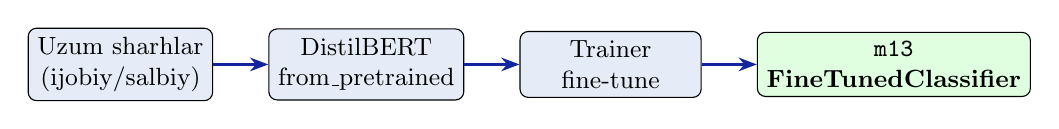
\begin{tikzpicture}[
      mod/.style={draw, fill=cnubluebg, rounded corners=3pt,
                  minimum width=2.3cm, minimum height=0.75cm,
                  font=\small, align=center},
      fin/.style={draw, fill=green!12, rounded corners=3pt,
                  minimum width=2.5cm, minimum height=0.75cm,
                  font=\small\bfseries, align=center},
      arr/.style={-{Stealth}, thick, color=cnublue}
  ]
    \node[mod] (op) {Uzum sharhlar\\ (ijobiy/salbiy)};
    \node[mod, right=0.7cm of op]  (be) {DistilBERT\\ from\_pretrained};
    \node[mod, right=0.7cm of be]  (ft) {Trainer\\ fine-tune};
    \node[fin, right=0.7cm of ft]  (m13) {\texttt{m13}\\ FineTunedClassifier};
    \draw[arr] (op)--(be); \draw[arr] (be)--(ft); \draw[arr] (ft)--(m13);
  \end{tikzpicture}
  \end{center}
  \vspace{5pt}
  \begin{columns}[T]
    \begin{column}{0.50\textwidth}
      \textbf{P13 da qurasiz:}\\[3pt]
      \small
      \begin{itemize}\setlength\itemsep{2pt}
        \item \texttt{m13 FineTunedClassifier}: BERT $+$ Trainer
        \item Uzum sentimentida fine-tuning (ijobiy/salbiy)
        \item BCE yo'qotish va baholash
      \end{itemize}
    \end{column}
    \begin{column}{0.46\textwidth}
      \textbf{Birinchi assert (bu slayd [I1]):}\\[4pt]
      \small\ttfamily
      assert abs(\\
      \phantom{xx}loss - 0.128) < 1e-2\\[4pt]
      \normalfont\footnotesize\color{halfgray}
      \textit{\# Ma'ruza L13 [I1]-slayd bilan}\\
      \textit{\# solishtiring (sigma(2.0), BCE)}
    \end{column}
  \end{columns}
\end{frame}

% ----------------------------------------------------------------
% [R] ADABIYOTLAR
% ----------------------------------------------------------------
\begin{frame}{Adabiyotlar}
  \begin{enumerate}\small\setlength\itemsep{5pt}
    \item Devlin, J., va boshq.\ (2019). \textit{BERT: Pre-training of Deep
          Bidirectional Transformers.} NAACL-HLT 2019.
    \item Raffel, C., va boshq.\ (2020). \textit{Exploring the Limits of Transfer
          Learning with a Unified Text-to-Text Transformer (T5).} JMLR 21.
    \item Howard, J., Ruder, S.\ (2018). \textit{Universal Language Model
          Fine-tuning (ULMFiT).} ACL 2018.
    \item Conneau, A., va boshq.\ (2020). \textit{Unsupervised Cross-lingual
          Representation Learning at Scale (XLM-RoBERTa).} ACL 2020.
    \item \texttt{huggingface.co/docs/transformers} hujjatlari.
  \end{enumerate}
\end{frame}

% ================================================================
% [S] ILOVALAR (appendix --- slayd soniga kirmaydi)
% ================================================================
\appendix

\begin{frame}{Ilova S1: MLM niqoblash strategiyasi (80/10/10)}
  \small
  BERT niqoblangan $15\%$ tokenni quyidagicha qayta ishlaydi:
  \begin{itemize}\setlength\itemsep{2pt}
    \item $80\%$ --- \texttt{[MASK]} bilan almashtiriladi.
    \item $10\%$ --- tasodifiy boshqa so'z bilan almashtiriladi.
    \item $10\%$ --- o'zgarishsiz qoldiriladi.
  \end{itemize}
  \bunda{Bu strategiya model fine-tuning paytida \texttt{[MASK]} ko'rmasligiga
  (train/test nomuvofiqligiga) qarshi turadi --- model har doim kontekstga tayanadi.}
\end{frame}

\begin{frame}{Ilova S2: T5 span-corruption pre-training}
  \small
  T5 alohida tokenlar emas, \textbf{bo'laklar} (span) ni niqoblaydi:
  $$ \text{kirish: } \texttt{"NLP <X> qiziq <Y> fan"} \;\to\;
     \text{chiqish: } \texttt{"<X> juda <Y> foydali"} $$
  \bunda{$\langle X\rangle, \langle Y\rangle$ --- maxsus sentinel tokenlar; model
  niqoblangan bo'laklarni ketma-ketlik sifatida tiklaydi --- bu enkoder-dekoder
  formatga tabiiy mos keladi.}
  \vspace{4pt}

  Shu tariqa T5 pre-training ham, fine-tuning ham bir xil matn$\to$matn shaklida bo'ladi.
\end{frame}

\end{document}
